%%%%%%%%%%%%%%%%%%%%%%%%%%%%%%%%%%%%%%%%%%%%%%%%%%%%%%%%%%%%%%%%%%%%%%%%%%%%%%%%
\chapter{Реализация генератора систем инструментирования}
%%%%%%%%%%%%%%%%%%%%%%%%%%%%%%%%%%%%%%%%%%%%%%%%%%%%%%%%%%%%%%%%%%%%%%%%%%%%%%%%

Программная реализация.

%%%%%%%%%%%%%%%%%%%%%%%%%%%%%%%%%%%%%%%%%%%%%%%%%%%%%%%%%%%%%%%%%%%%%%%%%%%%%%%%
\section{Синтез цепочек TXL функций}
%%%%%%%%%%%%%%%%%%%%%%%%%%%%%%%%%%%%%%%%%%%%%%%%%%%%%%%%%%%%%%%%%%%%%%%%%%%%%%%%

Поскольку язык, который используется для программирования утилиты TXL, принадлежит к семейству функциональных языков программирования, это ограничение заставляет передавать собираемую информацию посредством параметров, с которыми вызываются последующие функции в цепочке.

***

Цепочки вызовов функций запускаются посредством прямого вызова первых функций в каждой из функции главной функции с именем $main$, где  основным параметром всегда является корневой элемент конкретного дерева разбора с типом \textit{program}.
Результаты работы первой цепочки функций передаются далее одна за другой.

В листинге~\ref{main-example} приведен пример исходного текста функции $main$.
Символ ``...'' содержат имена функций, которые были сокращены для повышения удобочитаемости.

\begin{lstlisting}[frame=single, language=TXL, label={main-example}, caption={Пример исходного текста главной функции}]
function main
	replace [program]
		Program [program]
	by
		Program
		[..._refiner_imports_first0]
		[..._refiner_class_level0__helper]
		[..._collector_class_and_method_m_633_uid5]
		[..._collector_class_and_method_m_633_uid8]
		[simplify]
end function
\end{lstlisting}

Связывание нескольких TXL функций в единую последовательность было реализовано посредством наследования предметно-ориентированных типов функций от класса $CallChainElement$, описание которого приведено в листинге~\ref{chain-element-sample}.

\begin{lstlisting}[frame=single, language=C, label={chain-element-sample}, caption={Исходный код определения элемента цепочки вызовов}]
struct CallChainElement {
  /// calleR
  TXLFunction const* callFrom = nullptr;
  /// calleE
  TXLFunction const* callTo = nullptr;
}; // CallChainElement
\end{lstlisting}

***

Ниже представлена общая структура цепочки вызовов программно-синтезируемых предметно-ориентированных функций:
\begin{enumerate}[noitemsep]
  \item C-функции -- функции сбора информации.
  \item F-функции -- функции фильтрации.
  \item R-функций -- функций уточнения контекста.
  \item I-функции -- функции инструментирования.
\end{enumerate}

Кроме этого используются следующие вспомогательные автоматически-синтезируемые TXL функции:
\begin{itemize}
  \item G-функции -- функции получения узлов, содержащих полезные значения (так называемых \textit{точек интереса}), из промежуточных узлов дерева разбора, имеющих TXL тип, который описывает какую-либо важную синтаксическую конструкцию целевого языка программирования.
  \item H-функции -- функции проверки принадлежности определенному контексту по передаваемым параметрам.
  \item W-функции -- функции-обертки стандартных операторов сравнения и поиска, выполняемых над текстовыми данными.
\end{itemize}

***

%%%%%%%%%%%%%%%%%%%%%%%
\subsection{Функции сбора информации}
%%%%%%%%%%%%%%%%%%%%%%%

***

C-функции (англ. $collect$) -- это TXL функции, специализированные по типу обрабатывамых узлов дерева разбора, предназначенные для накопления информации из узлов древа разбора, которая впоследствии используется для определения, соответствует-ли рассматриваемый/обрабатываемый конечный узел дерева разбора выбранному контексту инструментирования.

Принцип работы таких функций заключается в вызове следующей функции из цепочки с передачей ей всех значений аргументов, которые были получены текущей, и текущего рассматриваемого узла, тип которого содержит необходимые сведения для дальнейших операций, таких как определение соответствия контексту и формирование значений для пользовательских переменных, используемых при заполнении исользуемого фрагмента исходного кода.

C-функции опираются на специфику работы функций-правил~(rule) языка TXL: правилу $R_{(T,P)}$ будут даны на рассмотрение все узлы текущего под-дерева $G_{sub}$, соответствующие заявленому типу $T$ и сопоставимые шаблону $P$.

В листинге~\ref{cfunc-example} приведен пример исходного TXL кода простой C-функции с именем \lstinline{CollectorFuncB}, которая получает в виде аргумента некоторый узел с типом \lstinline{class_declaration}, выполняет копирование обрабатываемого узла с типом \lstinline{method_declaration} и передает эти данные (два узла, переданный в аргументах и обрабатываемый) следующей функции по цепочке вызовов с именем \lstinline{CollectorFuncC}.

\begin{lstlisting}[frame=single, language=TXL, label={cfunc-example}, caption={Пример C-функции}]
rule CollectorFuncB kw_Class [class_declaration]
  skipping [method_declaration]
  replace $ [method_declaration]
    __NODE__ [method_declaration]
  by
    __NODE__ [CollectorFuncC kw_Class __NODE__]
end rule
\end{lstlisting}

Стоит отметить, что существуют разные подходы к решению задачи передачи информации по цепочке функций:
\begin {itemize}[noitemsep]
  \item аргументы функций
    \begin{itemize}[noitemsep]
      \item добавление новых аргументов в конец (слева-направо)
      \item добавление новых аргументов в начало (справа-налево)
    \end{itemize}
  \item глобальные переменные
  \item использование средств ввода-вывода среды TXL для временного хранения результатов во внешнем, родительском для утилиты TXL, процессе
\end{itemize}

Как видно из приведенного примера, для реализации прототипа был выбран первый способ передачи данных о необходимых узлах дерева разбора-- посредством аргументов функций, где новые узлы добавляются в конец.

***

%%%%%%%%%%%%%%%%%%%%%%%
\subsection{Функции фильтрации по контексту}
%%%%%%%%%%%%%%%%%%%%%%%

***

F-функции (англ. $filter$) -- это TXL функции, специализированные по типу обрабатывамых узлов дерева разбора, предназначенные для фильтрации узлов CST дерева разбора относительно описываемых конечным пользователем контекстов инструментирования.

В листинге~\ref{ffunc-example} приведен пример F-функции.

\begin{lstlisting}[language=TXL, label={ffunc-example}, caption={Пример F-функции}]
function filteringFunction kw_Class [class_declaration] kw_Method [class_declaration]
  skipping [method_declaration]
  replace $ [method_declaration]
    __NODE__ [method_declaration]
  construct __VOID__ [any]
    % void
  where
    __VOID__ [belongs_to_class_and_method kw_Class kw_Method]
  by
    __NODE__ [refinerFunction kw_Class kw_Method]
end function
\end{lstlisting}

***

%%%%%%%%%%%%%%%%%%%%%%%
\subsection{Функции уточнения контекста}
%%%%%%%%%%%%%%%%%%%%%%%

После проверки контекста функцией-фильтром, производится вызов первой функции из последовательности R-функций.

R-функции (англ. $refine$) -- это TXL функции, специализированные по типу обрабатывамых узлов дерева разбора, предназначенные для уточнения контекста...

В листинге~\ref{rfunc-example} приведен пример R-функции.

\begin{lstlisting}[frame=single, language=TXL, label={rfunc-example}, caption={Пример R-функции}]
function refinerFunction kw_Class [class_declaration] kw_Method [class_declaration]
  replace * [repeat declaration_or_statement]
    __NODE__ [if_statement] __TAIL__ [repeat declaration_or_statement]
  construct __SINGLE_BOX_ARRAY__ [repeat declaration_or_statement]
    __NODE__ % +empty
  construct __PROCESSED__ [repeat declaration_or_statement]
    __SINGLE_BOX_ARRAY__ [instrumentationFunction kw_Class kw_Method]
  by
    __PROCESSED__ [. __TAIL__]
end function
\end{lstlisting}

***

Вид и структуру порождаемой R-функции определяет используемый модицикатор, указываемый пользователем при составлении правил инструментирования.
Были реализованы следующие модификаторы для уточняющих функций:

\begin{itemize}[noitemsep]
  \item $first$ -- поиск и обработка \textit{только самого первого} встреченного узла из текущего поддерева разбора в соответствии с типом, заданным в аннотации грамматики при описании синтаксической конструкции целевого языка программирования.
  \item $all$   -- поиск и обработка \textit{всех узлов} в соответствии с типом, заданным в аннотации грамматики при описании синтаксической конструкции целевого языка программирования.
  \item $level$ -- поиск и обработка ***
\end{itemize}

На рисунках \ref{fig:modifier_level_a} и \ref{fig:modifier_level_b} показаны абстрактные примеры, демонстрирующие оказываемое модификатором $level$ влиянние на поведение уточняющей функции.
Красным цветом выделены ``целевые'' объекты, тип которых требуется обработать.
Жирным выделены только те объекты, которые соответствуют выражению ``\textit{первый уровень вложенности красных объектов друг в друга}''.

\begin{figure}[!h]
	\centering
	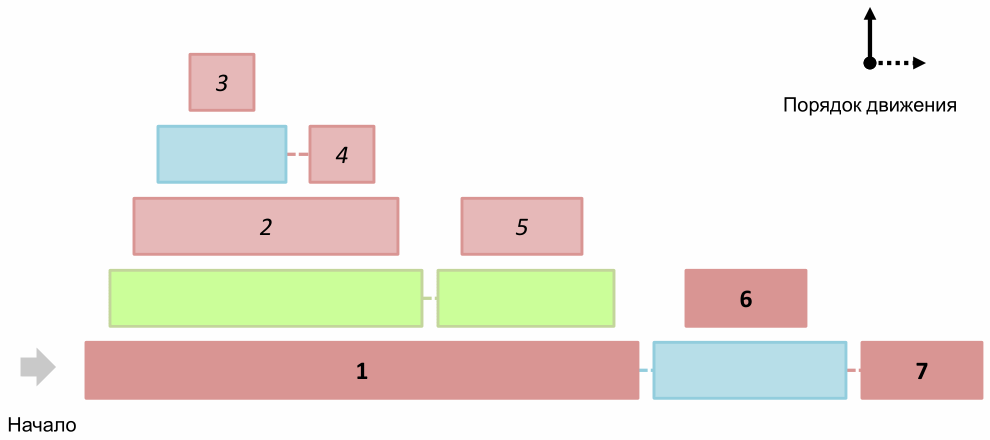
\includegraphics[width=3.2in]{modifier_level_a}
	\caption{Пример применения модификатора $level$.}
	\label{fig:modifier_level_a}
\end{figure}

\begin{figure}[!h]
	\centering
	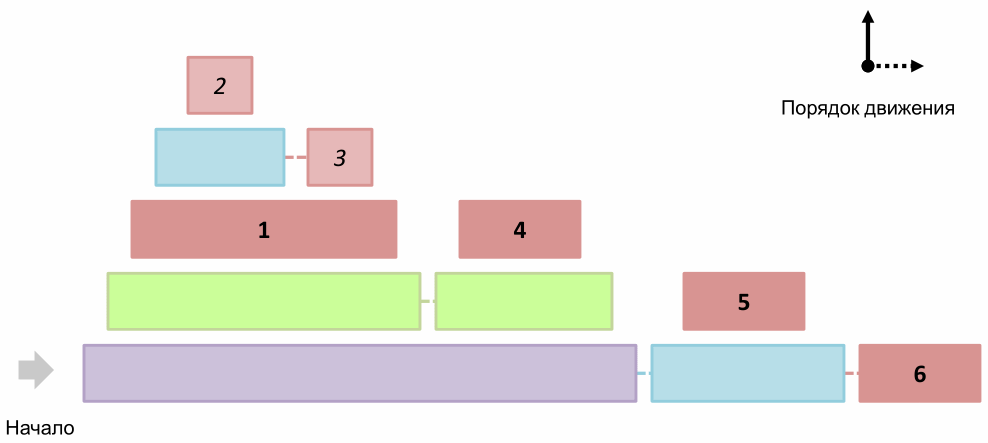
\includegraphics[width=3.2in]{modifier_level_b}
	\caption{Пример применения модификатора $level$.}
	\label{fig:modifier_level_b}
\end{figure}

***

Для каждой функции ренерируется вспомогательная ``стартовая'' функция, принимающая рассматриваемый уровнем выше узел и проводящая инициализацию переменной-счетчика для реализаций модификаторов типа $all$ и $level$.

***

Помимо модификаторов, R-функции способны осуществлять фильтрацию узлов на основании данных, извлекаемых из соответствующих точек интереса, которые были указаны при описании синтаксической конструкций целевого языка в аннотации грамматики.
Фильтрация осуществляется посредством проверки соответствия данных, представленных в точке интереса и текстового шаблона, задаваемого пользователем при составлении правил инструментирования.

В листинге ??? приведен пример использования модификаторов совместно с фильтрацией по шаблону.

***

%%%%%%%%%%%%%%%%%%%%%%%
\subsection{Функции инструментирования}
%%%%%%%%%%%%%%%%%%%%%%%

***

I-функции (англ. $instrument$) -- это TXL функции, специализированные по типу обрабатывамых узлов дерева разбора, предназначенные для инструментирования...

В листинге~\ref{ifunc-example} приведен пример I-функции.

\begin{lstlisting}[frame=single, language=TXL, label={ifunc-example}, caption={Пример I-функции}]
function instrumentationFunction kw_Class [class_declaration] kw_Method [class_declaration]
  replace [class_or_interface_body]
    __NODE__ [class_or_interface_body]
  deconstruct __NODE__
    '{ RepeatClassBodyDeclaration [repeat class_body_declaration] '} OptLiteral [opt ';]
  construct FILE [stringlit]
    _ [+ "*dir/test.java*"]
  construct POINTCUT [id]
    'all
  construct NODE [id]
    _ [typeof __NODE__]
  construct msg [stringlit]
    _  [quote POINTCUT] [+ " "] [quote NODE] [+ " block in "] [quote FILE] [+ " class, in "] [quote METHOD_NAME] [+ " method"]
  by
    'iLogger.log(Level.FINE, msg ');
    'if '( Condition ') '{ Statement '} OptElseClause
end function
\end{lstlisting}

***

%%%%%%%%%%%%%%%%%%%%%%%
\subsection{Вспомогательные TXL функции}
%%%%%%%%%%%%%%%%%%%%%%%

***

%%%%%%%%%%%
\subsubsection{H-функции}
%%%%%%%%%%%

***

H-функции (англ. $help$) -- это TXL функции, специализированные по типам обрабатывамых узлов дерева разбора, предназначенные для проверки принадлежности определенному контексту по передаваемым параметрам.

В листинге~\ref{hfunc-example} приведен пример H-функций с именами \lstinline{__belongs_to_context___namespace_m} и \lstinline{__not__belongs_to_context___namespace_m}.
Функция \lstinline{__belongs_to_context___namespace_m}, как видно из ее названия, реализует проверку принадлежности некоторого узла дерева разбора, который содержит данные с типом \lstinline{procedure_impl_decl} .

\begin{lstlisting}[frame=single, language=TXL, label={hfunc-example}, caption={Пример H-функции}]
function __belongs_to_context___namespace_m kw_Method [procedure_impl_decl]
	match [any]
		_ [any]
	construct __VOID__ [any]
		% void
	construct POI_METHOD_NAMESPACE_str [stringlit]
		_ [__POI_get___POI_METHOD_NAMESPACE kw_Method]
	where
		__VOID__ [__std__equal POI_METHOD_NAMESPACE_str "Main."]
end function


function __not__belongs_to_context___namespace_m kw_Method [procedure_impl_decl]
	match [any]
		_ [any]
	construct __VOID__ [any]
		% void
	where not
		__VOID__ [__belongs_to_context___namespace_m kw_Method]
end function
\end{lstlisting}

***

%%%%%%%%%%%
\subsubsection{G-функции}
%%%%%%%%%%%

***

G-функции (англ. $get$) -- это TXL функции, специализированные по типу обрабатывамых узлов дерева разбора, предназначенные для получения узлов, содержащих полезные значения, из промежуточных узлов дерева разбора, имеющих TXL тип, который описывает какую-либо важную синтаксическую конструкцию целевого языка программирования.

В листинге~\ref{gfunc-example} приведен пример G-функции.

\begin{lstlisting}[frame=single, language=TXL, label={gfunc-example}, caption={Пример G-функции}]
function __POI_get___POI_METHOD_NAME_FULL kw_Method [procedure_impl_decl]
	replace [stringlit]
		_ [stringlit]
	deconstruct kw_Method
		    ProcedureIntfDecl0 [procedure_intf_decl] _ [nested_decl_block] _ [procedure_body_semi]
	deconstruct ProcedureIntfDecl0
		    ProcedureSignature1 [procedure_signature] _ [repeat semi_directive] _ [opt ';]
	deconstruct ProcedureSignature1
		    _ [opt 'class] _ [procedure_keyword] ProcedureId2 [opt procedure_id] _ [opt formal_parameters] _ [opt colon_type]
	construct ProcedureId2_str [stringlit]
		_ [quote ProcedureId2]
	by
		ProcedureId2_str
end function
\end{lstlisting}

***

%%%%%%%%%%%
\subsubsection{W-функции}
%%%%%%%%%%%

***

W-функции (англ. $wrap$) -- это TXL функции, предназначенные для приведения стандартных операторов языка TXL, предназначенных для сравнения и поиска, и выполняемых над текстовыми/строковыми ($stringlit$ в текущей реализации прототипа) данными, из вида ``A~[op~B]'' (где $A$ -- имя некоторой переменной, $B$ -- значение или имя некоторой другой переменной, $op$ -- оператор сравнения), в котором один аргумент является основным аргументом функции-оператора сравнения, а второй -- второстепенным, в вид ``[op~A~B]'', что удобно при объединении операций сравнения в форму КНФ или ДНФ при выполнении проверок по нескольким критериям одновременно.
\nomenclature{КНФ}{коньюнктивная нормальная форма}
\nomenclature{ДНФ}{дизъюнктивная нормальная форма}

В листинге~\ref{wfunc-example} приведен пример исходного текста W-функции с именем \lstinline{__std__lower_equal}, которая используется для реализации обертки над операцией \textit{меньше или равно}.

\begin{lstlisting}[frame=single, language=TXL, label={wfunc-example}, caption={Пример W-функции}]
function __std__lower_equal A [stringlit] B [stringlit]
	match [any]
		_ [any]
	where
		A [<= B]
end function
\end{lstlisting}

***

Помимо стандартных операторов сравнения, таких как ``больше'', ``меньше'', ``равно'' и др., были реализованы следующие специальные опции:
\begin{itemize}[noitemsep]
  \item \textit{P has X} --
  текстовые данные, представленные в точке интереса $P$, сдержат в себе подстроку $X$. Текстовый фрагмент $X$ может как содержаться в начале, в середине и в конце проверяемого текста, так и повторяться неограниченное количество раз.

  \item \textit{P matches T} --
  текстовые данные, представленные в точке интереса $P$, соответствуют текстовому шаблону $T$. ***

  \item \textit{P exists} --
  явно указывает на необходимость существования в контексте инструментирования любых данных для выбранной точки интереса $P$, допустимых в соответствии с гамматикой языка программирования. Допустимым значением, относительно грамматики, может являться отсутствие значения, т.е. данные опциональны. Если отсутствие данных не помешает извлечь это опциональное значение, то в точке интереса $P$ будет содержаться пустая строка, иначе проверяемый узел дерева разбора будет удален из рассмотрения по причине несоответствия описываемому контексту. Использование этой опции не накладывает дополнительных ограничений на текстовое содержимое.
\end{itemize}

***

%%%%%%%%%%%%%%%%%%%%%%%%%%%%%%%%%%%%%%%%%%%%%%%%%%%%%%%%%%%%%%%%%%%%%%%%%%%%%%%%
\section{???}
%%%%%%%%%%%%%%%%%%%%%%%%%%%%%%%%%%%%%%%%%%%%%%%%%%%%%%%%%%%%%%%%%%%%%%%%%%%%%%%%

***

Команды, доступные пользователю (составителю аннотации) при описании алгоритма инструментирования в секции $algorithm$ аннотации грамматики.

\begin{itemize}[noitemsep]
  \item \lstinline{insert-text (text)} --
  вставка текста, заданного в параметре $text$, без экранирования в точке инструментирования, а именно, в выражении секции $by$ синтезируемой функции инструментирования (I-функции).

  \item \lstinline{insert-call (function, params)} --
  вставка вызова функции с именем $function$ с параметрами $params$, разделенными символом пробела. Параметры будут вставлены как есть, что позволяет использовать ключевое слово $each$ языка TXL для работы с последовательностями (массивами и списками).

  \item \lstinline{insert-fragment ([each-line-prefix], [each-line-postfix])} --
  вставка текста фрагмента в точке инструментирования. Для каждой строки текста фрагмента опционально может быть задан некоторый текст, добавляемый в начало \textit{each-line-prefix} и в конец \textit{each-line-postfix}.

  \item \lstinline{create-variable ([name], type, value)} --
  создание TXL переменной с типом $type$, значение которой задано текстом параметра $value$. Имя переменной будет сгенерировано автоматически из названия используемого типа, но также может быть указано вручную, используя параметр $name$.

  \item \lstinline{deconstruct-variable (type, variant)} --
  добавление в функцию инструментирования (I-функцию) конструкции TXL для декомпозиции переменной с типом $type$ в соответствии с грамматикой целевого языка программирования, используя вариант с номером $variant$, если TXL тип многозначен.

  \item \lstinline{fragment-to-variable (name, type, [each-line-prefix], [each-line-postfix])} --
  создание TXL переменной в теле I-функции с типом $type$ и именем $name$, которая содержит в себе текст добавляемого фрагмента программного кода. Как и функция \textit{insert-fragment}, команда позволяет для каждой строки добавляемого текста опционально задать ``префикс'' и ``суфикс''.
\end{itemize}

***

%%%%%%%%%%%%%%%%%%%%%%%
\subsection{Интерфейс командной строки}
%%%%%%%%%%%%%%%%%%%%%%%

***

Для реализации интерфейса командной строки, а именно разбора параметров запуска исполнимого модуля, при реализации прототипа генератора систем инструментирования были использованы возможности библиотеки $argparse$ \cite{argparse}.

\begin{itemize}
  \item \lstinline{--src filenameI.lang}                -- путь к исходному файлу с текстом инструментируемого программного обеспечения, написаном на выбранном (целевом) языке программирования.
  \item \lstinline{--dst filenameO.lang}                -- путь к файлу, в котором будет сохранен инструментированный текст программы.
  \item \lstinline{--rule filename.dsl}                 -- путь к файлу, в котором описываются пользовательские правила инструметирования.
  \item \lstinline{--annotation filename.xml}           -- путь к файлу, сожержащему аннотацию к грамматике, которая содержит описание конструкций языка программирования инструментируемого программного обеспечения.
  \item \lstinline{--fragments-dir /path/to/fragments/} -- путь к директории, который необходимо считать базовым при поиске используемых пользователем при описании правил инструментирования фрагментов текста на целевом языке программирования.

  \item \lstinline{--disable "rule_name_1;rule_name_2"} -- разделенный символом ``точка с запятой'' список названий пользовательских правил инструментирования, которые необходимо игнорировать при синтезе описания трансформаций для утилиты TXL.
  \item \lstinline{--no-cache}                          -- игнорировать ранее сохраненные результаты синтеза пользовательского набора правил, если таковые имеются.
  \item \lstinline{--txl-params}                        -- дополнительные параметры для утилиты TXL, передаваемые на завершающем этапе -- при выполнении трансформаций.

  \item \lstinline{--scis-grm-ruleset} -- путь к грамматике, которая на языке TXL описывает структуру файлов с пользовательскими правилами инструментирования.
  \item \lstinline{--scis-grm-txl}     -- путь к грамматике, которая на языке TXL описывает сам язык TXL.
\end{itemize}

Параметры \lstinline{--scis-grm-ruleset} и \lstinline{--scis-grm-txl} используются для сокращения числа обращений к файловой системе, если бы значения, задаваемые в этих параметрах, хранились бы в файлах настройки разработанного прототипа генератора систем инструментирования.

***

%%%%%%%%%%%%%%%%%%%%%%%%%%%%%%%%%%%%%%%%%%%%%%%%%%%%%%%%%%%%%%%%%%%%%%%%%%%%%%%%
\section{Выводы}
%%%%%%%%%%%%%%%%%%%%%%%%%%%%%%%%%%%%%%%%%%%%%%%%%%%%%%%%%%%%%%%%%%%%%%%%%%%%%%%%

Текст.
